\documentclass{article}

\usepackage{graphicx}
\usepackage{tikz}
\usepackage{tikzsymbols}
\usetikzlibrary{calc,patterns,shapes.geometric}
\pagestyle{empty}
\usepackage[margin=0pt]{geometry}
\geometry{papersize={14in,12in}}

\def\centerarc[#1](#2)(#3:#4:#5){\draw[#1] ($(#2)+({#5*cos(#3)},{#5*sin(#3)})$) arc (#3:#4:#5);}

\begin{document}
	\begin{figure}
		\centering
		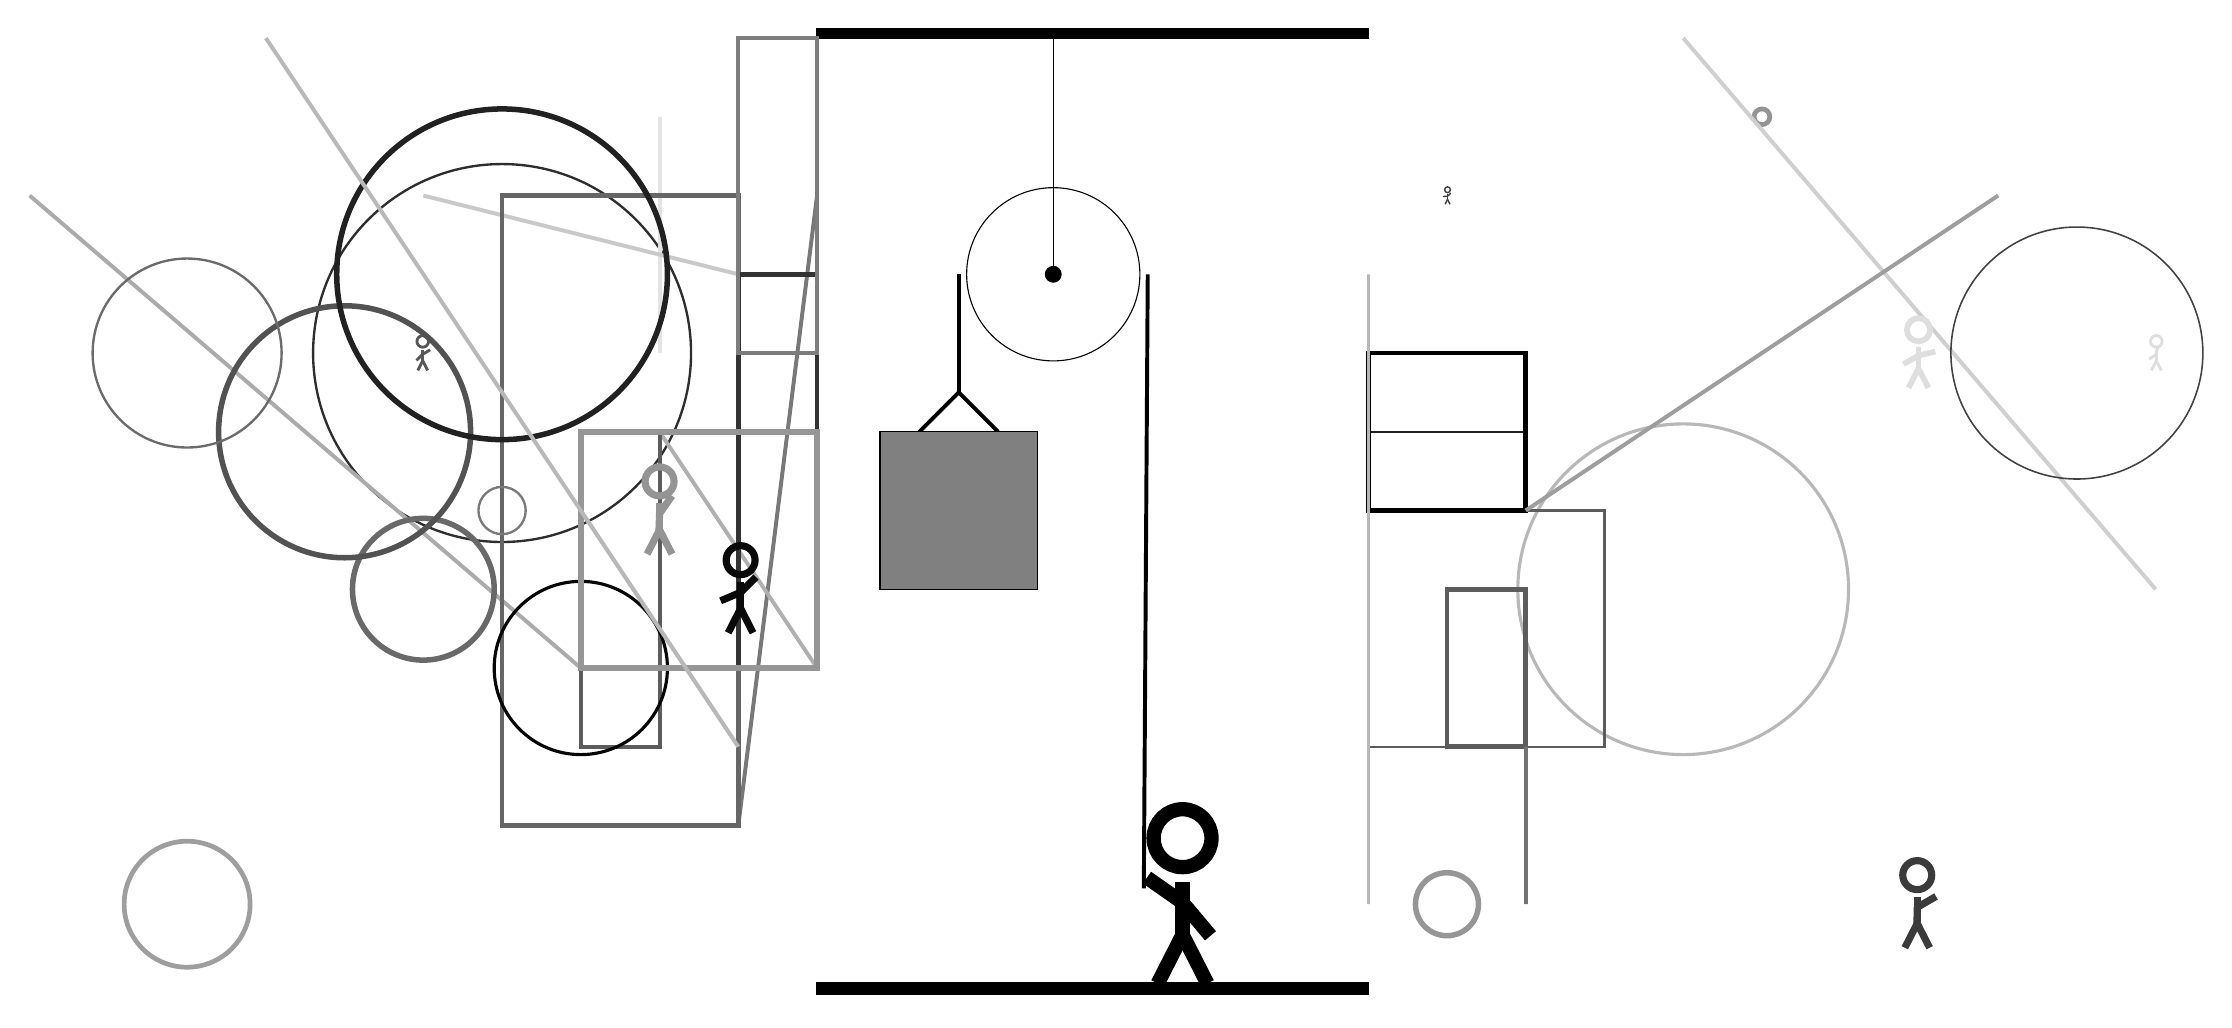
\begin{tikzpicture}
			%%%%% START %%%%%
			
			\draw[fill=black] (-2, 9) rectangle (5, 9.125);
			
			\draw (1, 6) circle (1.1);
			\draw[fill=black] (1, 6) circle (0.1);
			\draw (1, 9) -- (1, 6);
			
			\draw[line width=0.5mm] (-0.7, 4.0) -- (-0.2, 4.5) -- (0.3, 4.0);
			\draw[fill=black!50] (-1.2, 4.0) rectangle (0.8, 2.0);
			
			\draw[line width=0.5mm] (-0.2, 6) -- (-0.2, 4.5);
			\centerarc[line width=0.5mm](1, 6)(0:180:1.2000000000000002);
			\draw[line width=0.5mm](2.2, 6) -- (2.15, -1.8);
			
			\draw [line width=0.3mm, color=black!82](-6, 5) circle (2.4);
			
			\draw [line width=0.6mm, color=black!42](10, 8) circle (0.1);
			\node[line width=0.5mm, color=black!66] at (-7, 5) {\Strichmaxerl[2][44][31]};
			\draw[line width=0.5mm, color=black!11] (-4, 5) rectangle (-4, 8);
			
			\draw[line width=0.2mm, color=black!87] (5, 4) rectangle (7, 5);
			\draw [line width=0.7mm, color=black!41](6, -2) circle (0.4);
			\draw[line width=0.5mm, color=black!33](-5, 1) -- (-12, 7);
			
			\draw[line width=0.5mm, color=black!70](7, -2) -- (7, -2);
			\draw[line width=0.5mm, color=black!53](-2, 7) -- (-3, -1);
			
			\draw [line width=0.7mm, color=black!59](-7, 2) circle (0.9);
			\draw[line width=0.5mm, color=black!31](-4, 4) -- (-2, 1);
			
			\draw[line width=0.5mm, color=black!14](-3, 0) -- (-5, 3);
			\draw[line width=0.5mm, color=black!21](-3, 6) -- (-7, 7);
			
			\draw[line width=0.5mm, color=black!64] (-4, 4) rectangle (-5, 0);
			\draw [line width=0.4mm, color=black!28](9, 2) circle (2.1);
			\draw[line width=0.6mm, color=black!60] (-3, 7) rectangle (-6, -1);
			\draw [line width=0.3mm, color=black!52](-6, 3) circle (0.3);
			\draw[line width=0.5mm, color=black!19](9, 9) -- (15, 2);
			\draw[line width=0.6mm, color=black!64] (6, 2) rectangle (7, 0);
			\node[line width=0.6mm, color=black!13] at (15, 5) {\Strichmaxerl[2][34][80]};
			\node[line width=0.5mm, color=black!75] at (6, 7) {\Strichmaxerl[1][5][43]};
			\draw[line width=0.6mm, color=black!80] (-3, 6) rectangle (-2, 1);
			
			\draw[line width=0.3mm, color=black!64] (5, 3) rectangle (8, 0);
			\node[line width=0.5mm, color=black!96] at (-3, 2) {\Strichmaxerl[5][23][45]};
			\draw [line width=0.7mm, color=black!68](-8, 4) circle (1.6);
			\draw [line width=0.3mm, color=black!58](-10, 5) circle (1.2);
			\draw [line width=0.4mm, color=black!98](-5, 1) circle (1.1);
			\draw [line width=0.2mm, color=black!74](14, 5) circle (1.6);
			
			\draw[line width=0.5mm, color=black!55] (7, 0) rectangle (7, -2);
			\draw[line width=0.6mm, color=black!100] (5, 5) rectangle (7, 3);
			\draw[line width=0.5mm, color=black!38](7, 3) -- (13, 7);
			
			\draw [line width=0.6mm, color=black!38](-10, -2) circle (0.8);
			\draw[line width=0.7mm, color=black!41] (-2, 4) rectangle (-5, 1);
			
			\node[line width=0.6mm, color=black!42] at (-4, 3) {\Strichmaxerl[5][88][55]};
			
			\node[line width=0.4mm, color=black!77] at (12, -2) {\Strichmaxerl[5][89][30]};
			\draw[line width=0.5mm, color=black!51] (-2, 5) rectangle (-3, 9);
			
			\draw[line width=0.4mm, color=black!28] (5, -2) rectangle (5, 6);
			
			\draw [line width=0.7mm, color=black!87](-6, 6) circle (2.1);
			\draw[line width=0.5mm, color=black!28](-3, 0) -- (-9, 9);
			\node[line width=0.2mm, color=black!13] at (12, 5) {\Strichmaxerl[4][30][13]};
			
			\node at (2.6, -1.9) {\Strichmaxerl[10][-35][-50]};
			
			\draw[fill=black] (-2, -3) rectangle (5, -3.15);
			
			%%%%% END %%%%%
		\end{tikzpicture}
	\end{figure}	
\end{document}